\documentclass[12pt]{article}
\usepackage[utf8]{inputenc}
\usepackage{manfnt}
\usepackage{amsfonts}
\usepackage[margin=2cm]{geometry}
\usepackage[spanish]{babel}
\usepackage{graphicx}
\usepackage{tikz,pgfplots}
\usepackage{amsmath}

\begin{document}
	\title{Segundo Proyecto de Programaci\'on Declarativa}
	\author{Carlos Toledo Silva C-311\\
		    Ariel A. Triana P\'erez C-311}
	\date{}
	\maketitle
	
\section{Introducci\'on}

En el siguiente documento se realizar\'a la presentaci\'on de la aplicaci\'on Loki Text Adventure. Para esto dividiremos el resto del documento en secciones. En una primera secci\'on estaremos hablando sobre la historia elaborarda para la aplicaci\'on y en una posterior secci\'on nos referiremos a como un usuario interact\'ua con la aplicaci\'on. Posteriormente nos estaremos refiriendo a la implementaci\'on de la aplicaci\'on: estrategia que se sigui\'o, descripci\'on de los m\'odulos implementados y como se aprovecharon las caracter\'isticas propias de Haskell para dicha implementaci\'on.

\section{Historia elaborada para la aplicaci\'on}

La hostoria que se narra en la aplicaci\'on est\'a basada en la mitolog\'ia n\'ordica. El usuario asume el papel de Loki: un dios embaucador de esta mitolog\'ia y uno de los dioses m\'as conocidos. El usuario, metido en el papel de Loki, tomar\'a parte en una historia en la que pasar\'a por diferentes aventuras y dificultades, donde las decisiones que tome y los actos que realicen tendr\'an una influencia directa en la historia del mundo.

V\'alido aclarar que aunque la historia est\'a basada en la mitolog\'ia n\'ordica, muchos de los pasajes que en ella se narran no ocurren exactamente igual, ni siquiera en el orden correspondiente a como est\'an realmente recogidos en la mitolog\'ia. Otros muchos ni siquiera ocurrieron y son invenci\'on de los autores. De esta forma se ha adaptado la historia de Loki y otros personajes n\'ordicos para lograr hacer una historia entretenida y atractia para el usuario.

La historai est\'a compuesta de 3 cap\'itulos, seguidos uno a continuaci\'on del otro. Es decir que para el usuario poder llegar el cap\'itulo $i+1$ deber\'a haber triunfado en el cap\'itulo $i$. Adem\'as cada cap\'itulo cuenta con varios finales; en algunos el jugador sale triunfante pero en otros le podr\'ia acabar perdiendo la vida. Por esto motivo el jugador deber\'a escoger sabiamente, si es que quiere avanzar lo m\'as posible.  

\section{Interacci\'on entre el jugador y la aplicaci\'on}

Cuando se ejecuta la aplicaci\'on (ya compilada) lo primero que se ve es lo siguiente:

\begin{figure}[h]
	\begin{center}
		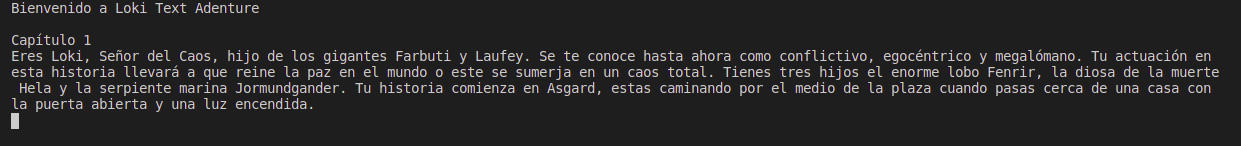
\includegraphics[width =15.0cm]{Inicial.png}
	\end{center}
\end{figure}

Aqu\'i es donde comienza la historia. A medida que el personaje avance en la historia le ir\'an saliendo texto similares a estos. Para poder avanzar el usuario deber\'a utilizar la informaci\'on mostrada en cada uno de los textos y dar una respuesta l\'ogica y bien escrita mediante alguna acci\'on. Es importante recalcar que las acci\'on se deben expresar mediante infinitivos: entrar, aceptar, hablar, etc y que por supuesto estos se combinen con las otras palabras necesarias para elaborar una idea coherente. Tambi\'en es importante recalcar que las acciones sobre el propio jugador deben ir seguidas del pronombre personal me; ejemplo: transformarme, quedarme, etc.

Por ejemplo partiendo del texto inicial podemos hacer lo siguiente:
\begin{figure}[h]
	\begin{center}
		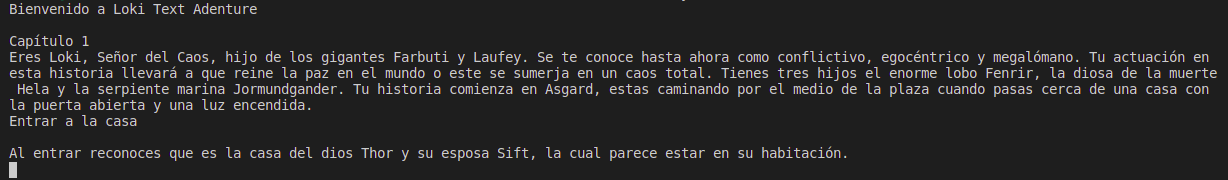
\includegraphics[width =15.0cm]{Avance.png}
	\end{center}
\end{figure}

Obs\'ervese como al escribir una acci\'on l\'ogica correctamente hemos avanzado en la historia. Si por el contrario escribimos una acci\'on sin sentido o no escrita correctamente (ya sea por palabras incorrectamente escritas o falta de las mismas), la aplicaci\'on puede que no reconozca lo que el usuario quiere decir y si esto pasa alertar\'a de esto y volver\'a a imprimir el \'ultimo texto impreso. A continuaci\'on mostramos un ejemplo:

\begin{figure}[h]
	\begin{center}
		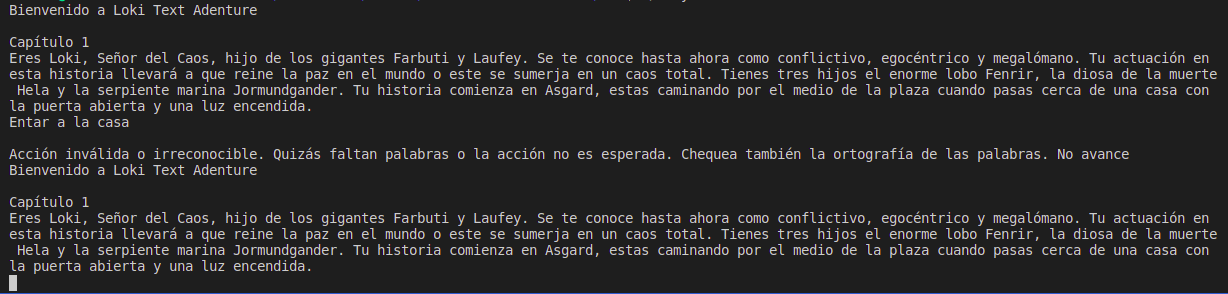
\includegraphics[width =15.0cm]{No_avance.png}
	\end{center}
\end{figure}

F\'ijese que cuando sali\'o el cartel por primera vez el usuario escribi\'o mal la palabra "Entrar" y por este motivo la acci\'on no se pudo reconocer. 

Tambi\'en durante el juego aparecer\'an situaciones en las que el usuario tendr\'a que escoger entre varias opciones. De esta forma la aplicaci\'on posibilita que el usuario pueda transitar por diferentes pasajes en base a sus decisiones. Cuan larga pueda ser la experiencia del jugador, tambi\'en depender\'a de las decisiones que tome. Una ''mala'' decisi\'on, por decirlo de alguna forma, podr\'ia provocar que el usuario terminar\'a el juego antes de terminar los 3 cap\'itulos. Veamos un ejemplo donde el usuario se enfrenta a una decisi\'on: 

\begin{figure}[h]
	\begin{center}
		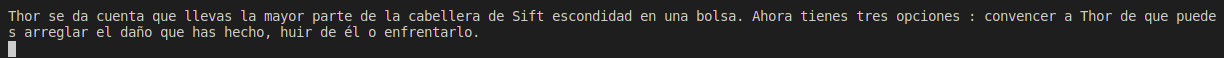
\includegraphics[width =15.0cm]{Decision.png}
	\end{center}
\end{figure}

En este caso el jugador podr\'a escoger entre convencer, hablar o enfrentar a Thor. En dependencia de lo que teclee el usuario se mover\'a a uno u otro pasaje.

\section{Implementaci\'on}

\subsection{Estrategia de implementaci\'on}

Como toda historia, esta est\'a compuesta por diferentes pasajes. Por este motivo definimos un tipo ''passage'' para representar los diferentes pasajes. M\'as adelante veremos como est\'a implementado este tipo. En todo momento el jugador se va encontrar transitando en un determinado pasaje. Para cambiar de pasaje, lo cual provoca un avance en la historia, el jugador teclea una sentencia, a la cual se realiza un an\'alisis para determinar si se cambia a alg\'un otro pasaje o si la historia se mantiene en el mismo. Cuando se alcanza alg\'un pasaje ''final'' la ejecuci\'on de la aplicaci\'on se detiene.

\subsection{M\'odulos implementados}

La implementaci\'on de la aplicaci\'on, para mejor organizaci\'on y comprensi\'on, est\'a dividida en los siguintes m\'odulos: ''Passages'', ''Synonyms'',''Functions'' y ''Loki-Text-Adenture''. En el m\'odulo ''Passages'' est\'a implementada la definici\'on de el tipo ''Passage'', el m\'odulo ''Functios'' se est\'a la implementaci\'on de las funciones que permiten llevar el pasaje actual, el an\'alisis de la entrada del usuario y el cambio o no de un pasaje a otro. Finalmente est\'a el m\'odulo principal ''Loki-Text-Adevneture'' que apoy\'andose de los otros m\'odulos permite el funcionamiento de la aplicaci\'on. A continuaci\'on veremos estos m\'odulos por separado 

\subsubsection{M\'odulo Passages}

Como se mencion\'o anteriormente, en este m\'odulo est\'a definido el tipo ''Passage'' del cual veremos ahora su definici\'on.

\begin{figure}[h]
	\begin{center}
		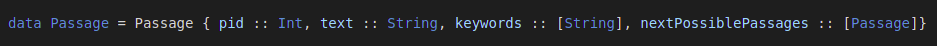
\includegraphics[width =15.0cm]{Passage.png}
	\end{center}
\end{figure}

El entero ''pid'' lo utilizamos para comparar pasajes de una forma eficiente. El string ''text'' es el texto correspondiente a un pasaje. Esto es lo que se imprime en pantalla cuando se llega a dicho pasaje. La lista de Passage ''nextPossiblePassages'' son los pasajes a los cuales se puede avanzar a partir del pasaje actual. La lista de string ''keywords'' son las palabras que debe teclear el usuario (o algunas que sean sin\'onimos de estas o que transmitan una idea similar) que permiten a partir de un pasaje espec\'ifico alcanzar el pasaje con esas keywords. O sea si yo el usuario se encuentra en el pasaje $i$ y en la lista ''nextPossiblePassages'' del pasaje $i$ se encuentra el pasaje $j$, par que el usuari\'o pueda pasar del pasaje $i$ al pasaje $j$ deber\'a teclear las palabras que aparecen en la lista ''keywords'' del pasaje $j$ (o algunas que sean sin\'onimos de estas o que transmitan una idea similar). De esta forma es que ocurre el cambio entre pasajes.

De la forma antes descrita, aparecen adem\'as definidos todos los pasajes de la historia. El pasaje inicial es el \'unico que tiene su lista ''keywords'' vac\'ia pues este no se alcanza desde ning\'un otro pasaje. Los pasajes finales, o sea los que no permitan avanzar al jugador m\'as all\'a de ellos, se caracterizan porque su lista de pasajes ''nextPossiblePassages'' es una lista vac\'ia.

\subsubsection{M\'odulo Synonyms}

\subsubsection{M\'odulo Functions}

En este m\'odulo se encuentran definidas las funciones que permiten el correcto funcionamiento de la aplicaci\'on.

La funci\'on ''actualPassage'' permite la creaci\'on de una variable global en la que se guardar\'a en todo momento el pasaje en el cual se encuentra la historia. 

La funci\'on ''changePassage'' recibe como par\'ametro un ''Passage'' y lo que hace es definir al pasaje actual como el pasaje que se le pasa de entrada.

La funci\'on ''obtainPassage'' se utiliza para poder obtener el pasaje actual en el que se encuentra la historia.

\subsubsection{M\'odulo Loki-Text-Adventure}

Este es el m\'odulo principal de la aplicaci\'on. En este m\'odulo primero tenemos dos funciones ''isWindows'' y ''setEncoding''. La primera la utilizamos para saber si la aplicaci\'on se est\'a ejecutando en Windows o no. La segunda es se utiliza para cambiar en el formato de codificaci\'on de caracteres a UTF-8 en caso de que no estemos en Windows. Esto lo hacemos porque nos paso que uno de nostros program\'o en Windows 10 y el otro en Ubuntu 18.04 y si no cambiamos el formato de codificaci\'on de caracteres en Ubuntu la aplicaci\'on no reconoc\'ia los caracteres del Español como las tildes y la ñ. Sin embargo si cambiamos esta codificaci\'on en Windows ocurr\'ia entonces que dichos caracteres no se reconoc\'ian y al no cambiarlo si lo hac\'ian. Por tanto se opt\'o por comprobar si se estaba ejecutando la aplicaci\'on en Windows para cambiar o no la configuraci\'on de codificaci\'on de caracteres.

\end{document}